
To prepare the data for training, we follow a structured preprocessing pipeline that ensures clean and well-formatted input sequences.
The first step involves retrieving and cleaning the DadaGP dataset, extracting tokens specific to selected instruments while preserving relevant note effect tokens and metadata.
We then apply an existing method to detect rhythm guitar parts within the dataset, selecting the most rhythmic guitar track for conditioning bass guitar generation.  
Next, we segment the extracted tokens into overlapping sequences of 16 measures with a stride of 8, applying length constraints to remove excessively long or short sequences.
The selected sequences are then formatted into structured dictionaries, where rhythm guitar tokens are used as encoder inputs, and bass guitar tokens serve as decoder targets.  
Finally, the sequences are converted to token indices, padded to fixed lengths, and split into training, validation, and test sets for model development and evaluation.
The following subsections provide a detailed explanation of each of these steps.  

\subsection{DadaGP token preprocessing}
% --> Retrieving, cleaning, mapping DadaGP
% Rhythm guitar detection (cite paper)

The DadaGP dataset provides token files containing information for all instruments in a score.
As we want to explore various conditioning combinations for tablature generation, we developed a function to extract tokens specific to selected instruments.
We considered several possible ways to perform this extraction: runnning DadaGP's token processing script for each instrument, or filtering the tokens from the complete token text file based on the instrument name.
Opening, parsing and looping on the GuitarPro file using \texttt{pyGuitarPro}\footnote{https://pyguitarpro.readthedocs.io/en/stable/} is needed for the DadaGP token processing script and is very time-consuming, much more than processing text files.
To perform the extraction of instrument-specific tokens, we use the filtering method from the existing token text files.
We leverage the fact that tokens of a given instrument start with the instrument name followed by a colon, e.g., \texttt{bass:} for the bass guitar.
However we must be careful not to miss the potential note effect tokens that are not instrument-specific, but come right after the token they are related to.
After extracting those tokens and the general tokens (metadata tokens and wait tokens),
we sum the potential consecutive wait tokens that were previously separated by notes from instruments that are no longer present.
This process took 5min30 on the 26,181 GuitarPro files of DadaGP to generate a copy of the dataset containing token files of bass guitar only.

\begin{figure}[!ht]
    \centering
    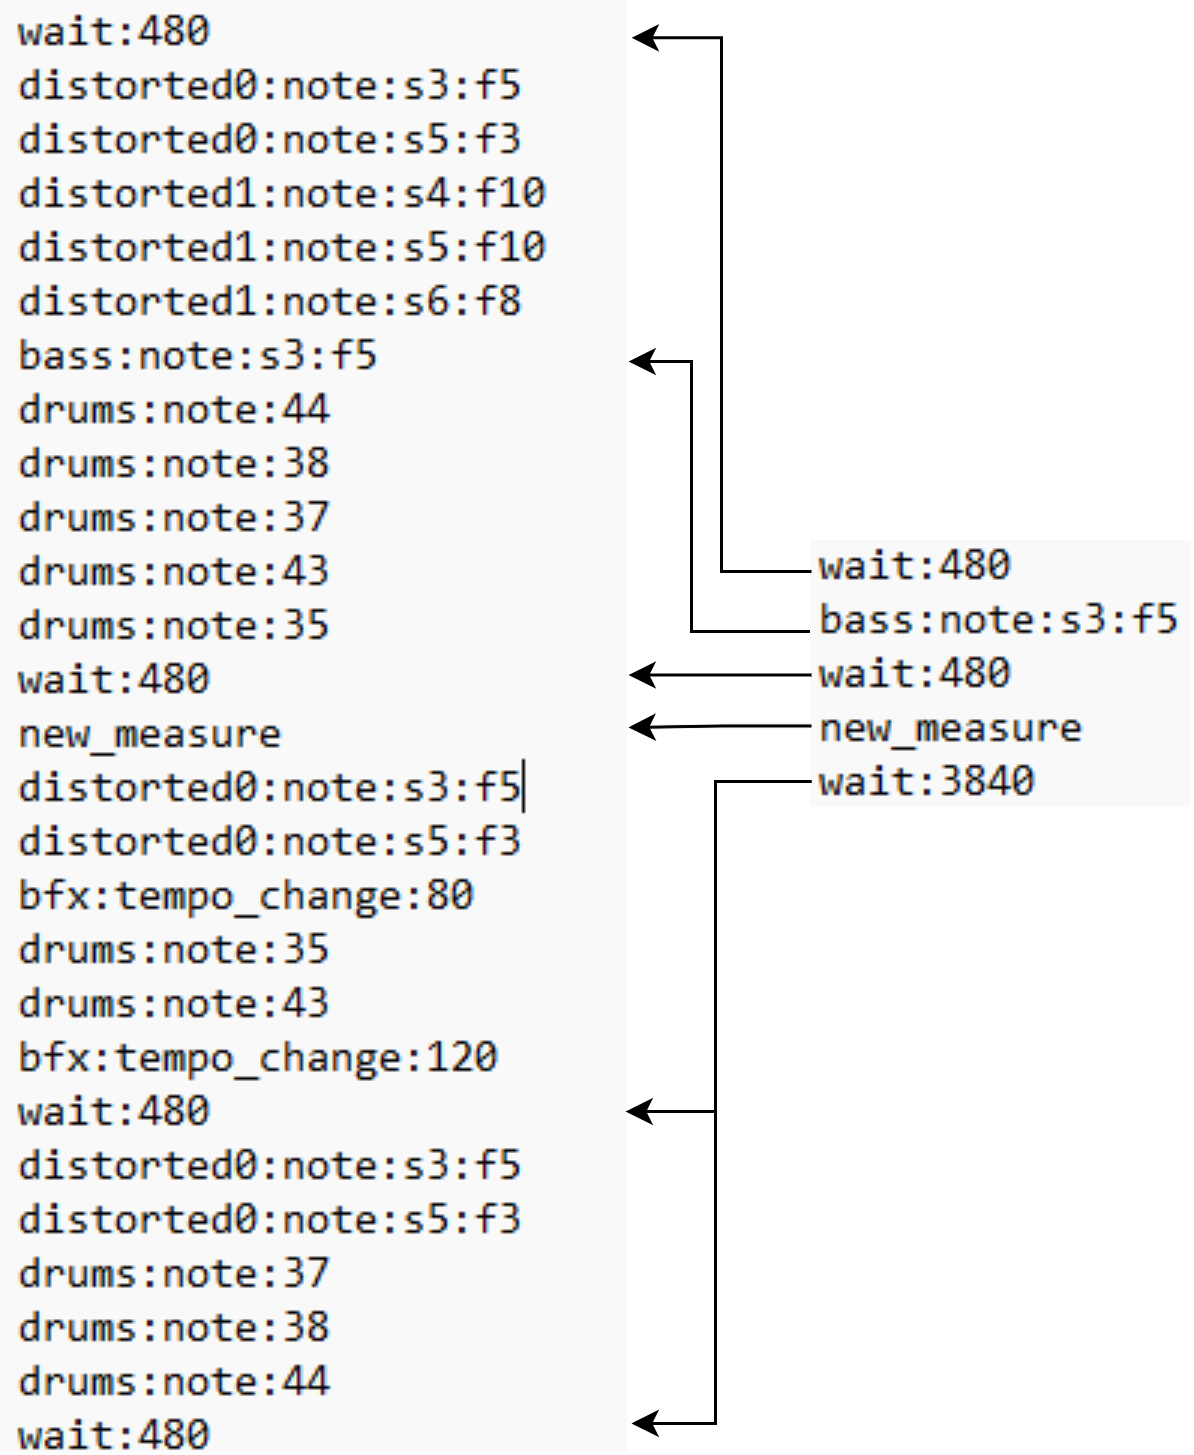
\includegraphics[width=.4\linewidth]{../images-figures/token_extraction.png}
    \caption{Example of an extraction of bass guitar token in The Strokes - Last Nite}
    \label{fig:token_extraction}
\end{figure}

An example of token extraction is shown in Figure~\ref{fig:token_extraction}.
Note from \texttt{distorted0}, \texttt{distorted1} and \texttt{drums} are removed as well as \texttt{bfx} tokens.
This figure also shows the concatenation of wait tokens, at the end of the song the bass guitar stops playing before the other instruments.
Therefore, we can notice that eight \texttt{wait:480} tokens (some are not shown here) are summed up to a single \texttt{wait:3840} token.



\subsection{Rhythm guitar identification}

The algorithm we just presented allows us to extract tokens for any instrument in the DadaGP dataset.
In typical rock band instrumentation, rhythm guitars complement bass guitars with their repetitive chord patterns, providing harmonic and rhythmic structure at a higher pitch~\cite{regnier_identification_2021}.
This characteristic makes them particularly relevant for conditioning bass generation tasks. Therefore, our first focus is on conditioning bass guitar tablature generation using the rhythm guitar.
However, as part of the rhythm section, drums and bass also form a crucial pair in the band.
Conditional generation using the drums part was considered, but the absence of pitch and harmonic information in drums made it less relevant for our task.


To identify rhythm guitar parts in the DadaGP dataset, we implemented the method proposed by Régnier et al.~\cite{regnier_identification_2021},
which uses features describing notes and chords at the bar level, along with corresponding tablatures.
Their model outputs a prediction between 0 and 1 for each bar. The closest to 1, the more likely the bar is to be lead guitar, and the closest to 0, the more likely the bar is to be rhythm guitar.
In their paper, they consider that a score below 0.5 correspond to a rhythm guitar parts.
As instrumentation can greatly vary between songs and genres, we wanted to select and condition the generation on only one guitar part, the ``most" rhythmic among the guitar parts present.
Therefore, we applied the 0.5 threshold to the predictions and selected the part with the highest proportion of rhythmic bar over the course of the song.
Implementing this method required adapting their code to the DadaGP dataset.
Significant effort was spent mapping the identified rhythm guitar parts to their respective names in the DadaGP files, as the dataset renames instruments, whereas the identification tool relies on GuitarPro part names.
Thanks to this work, we were able to extra  ct two more datasets: one containing the rhythm guitar tokens and the other containing both the bass and the rhythm guitar tokens.

% FIGURE EXAMPLE OF SELECTION OF RHYTHM GUITAR ON A SONG
\begin{figure}[!ht]
    \centering
    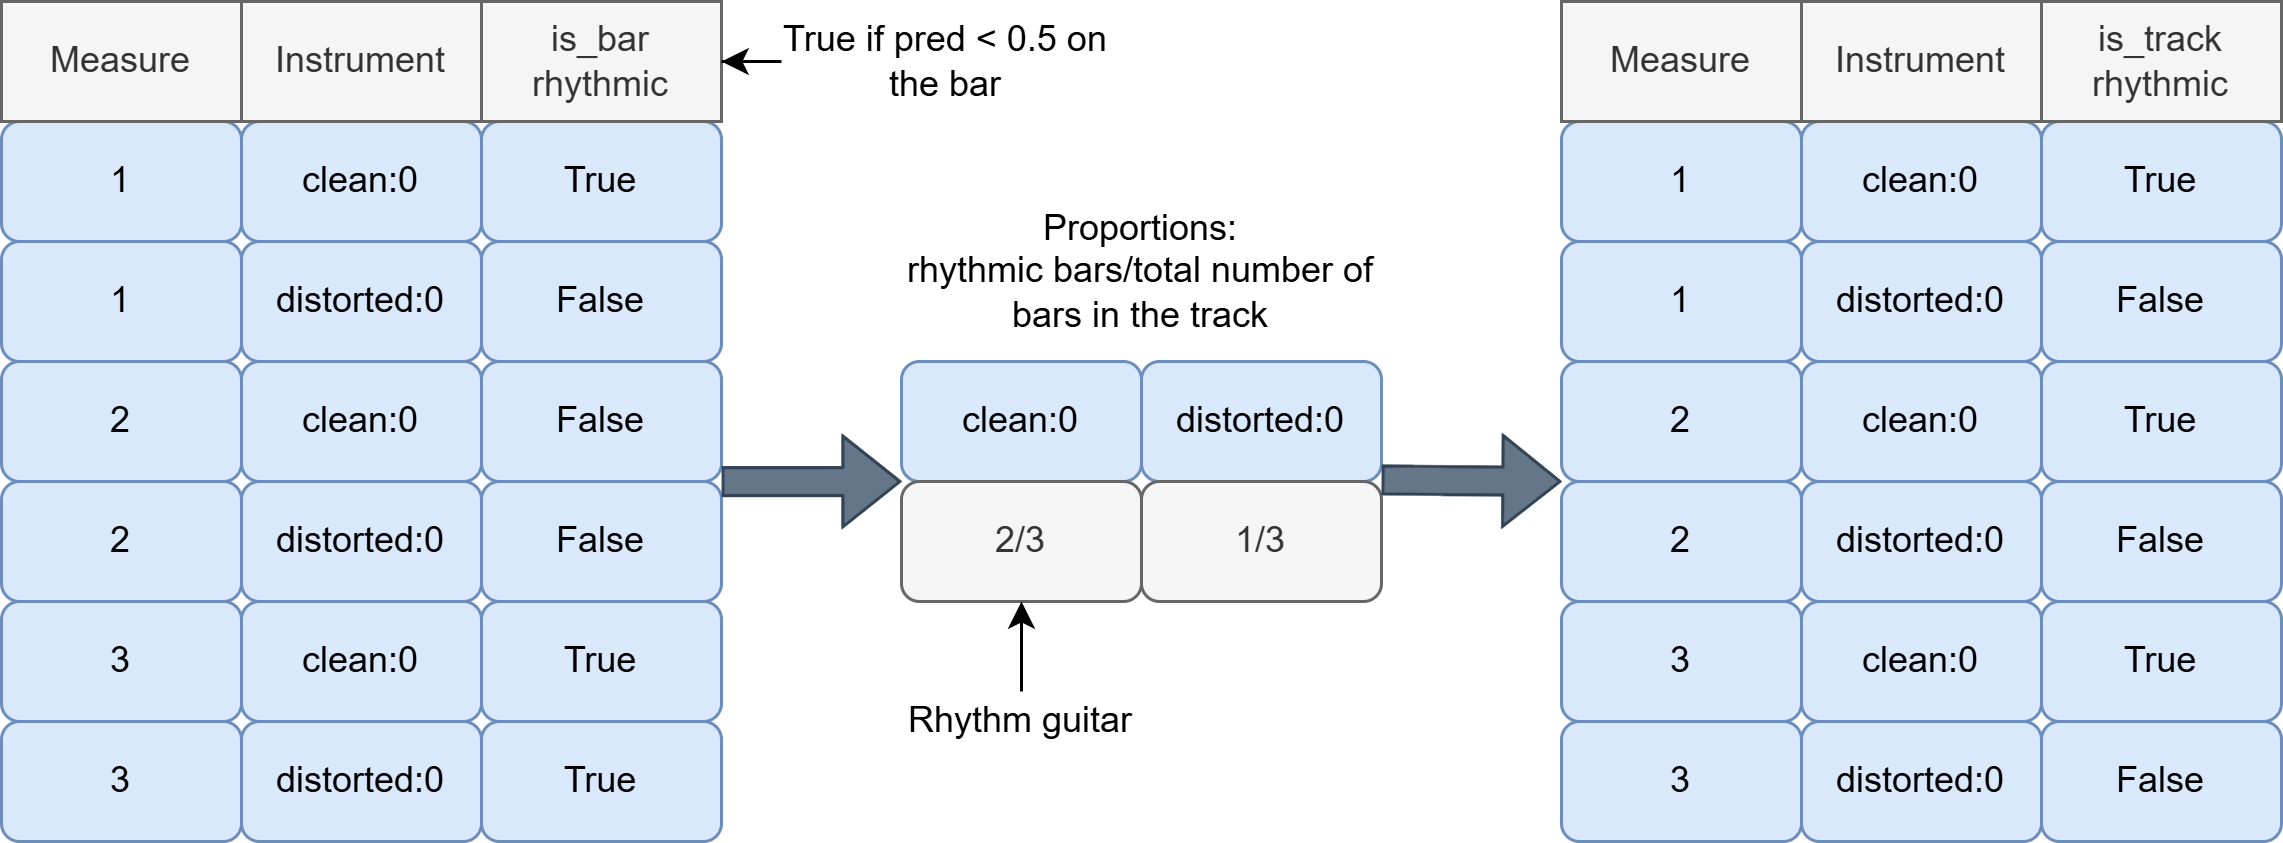
\includegraphics[width=0.85\linewidth]{../images-figures/rhythm_guitar_selection.png}
    \caption{Example of rhythm guitar selection after applying the method of Régnier et al.}
    \label{fig:rhythm_guitar_selection}
\end{figure}

Figure~\ref{fig:rhythm_guitar_selection} shows an example of the selection of the rhythm guitar part.
After retrieving the instrument with the highest number of rhythmic bars over the song,
we generate a column \texttt{is\_track\_rhythmic} that is filled with 1 (or True) for the rhythm guitar and 0 for the other instruments.


\subsection{Post processing}

To avoid sequences that are too long, we chose to extract samples of 16 measures from the songs.
We extract sequences with a stride of 8 measures, which allows us to have a good overlap between the sequences.
This will help the model to learn the transitions, and understand the various possible contexts around a given sequence.

% FIGURE DISTRIBUTION OF SEQUENCE LENGTHS
\begin{figure}[!ht]
    \centering
    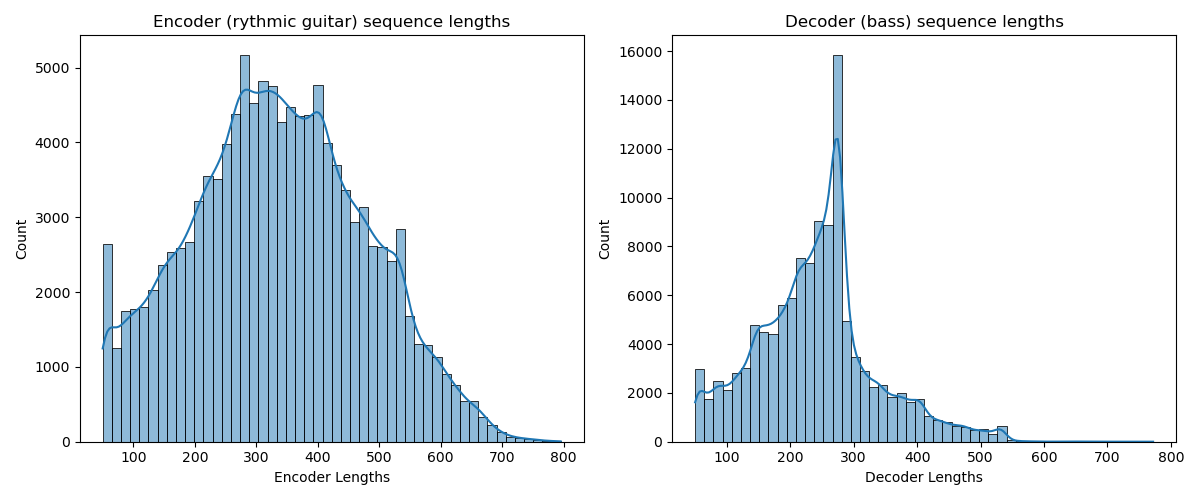
\includegraphics[width=.8\linewidth]{../images-figures/sequence_lengths_16_8_800_50.png}
    \caption{Distribution of sequence lengths in the training dataset}
    \label{fig:sequence_length_distribution}
\end{figure}

A maximum threshold of 800 tokens, and a minimum threshold of 50 tokens were set to avoid training on sequences that are either too long or that does not contain rythmic guitar or bass.
These are not applied on the complete sequences containing both the tokens of the rhythm guitar and the bass.
Figure~\ref{fig:sequence_length_distribution} shows the distribution of sequence lengths in the training dataset.
The majority of the sequences are between 200 and 400 tokens long for the rythmic guitar and between 100 and 300 tokens long for the bass.
Then, the sequences are fitted to the model's input requirements using an adapted version of the processing process of Makris et al.~\cite{makris_conditional_2022}.
The sequences fill in a dictionary with keys \texttt{Encoder\_RG}, \texttt{Decoder\_Bass} and \texttt{All\_Events}.
For instance \texttt{dict}[\texttt{Encoder\_RG}][i] contains the tokens of the rhythm guitar for the i-th sequence.
\texttt{dict}[\texttt{All\_Events}][i] contains the tokens of bass guitar and rhythm guitar for the i-th sequence.


\begin{figure}[!ht]
    \centering
    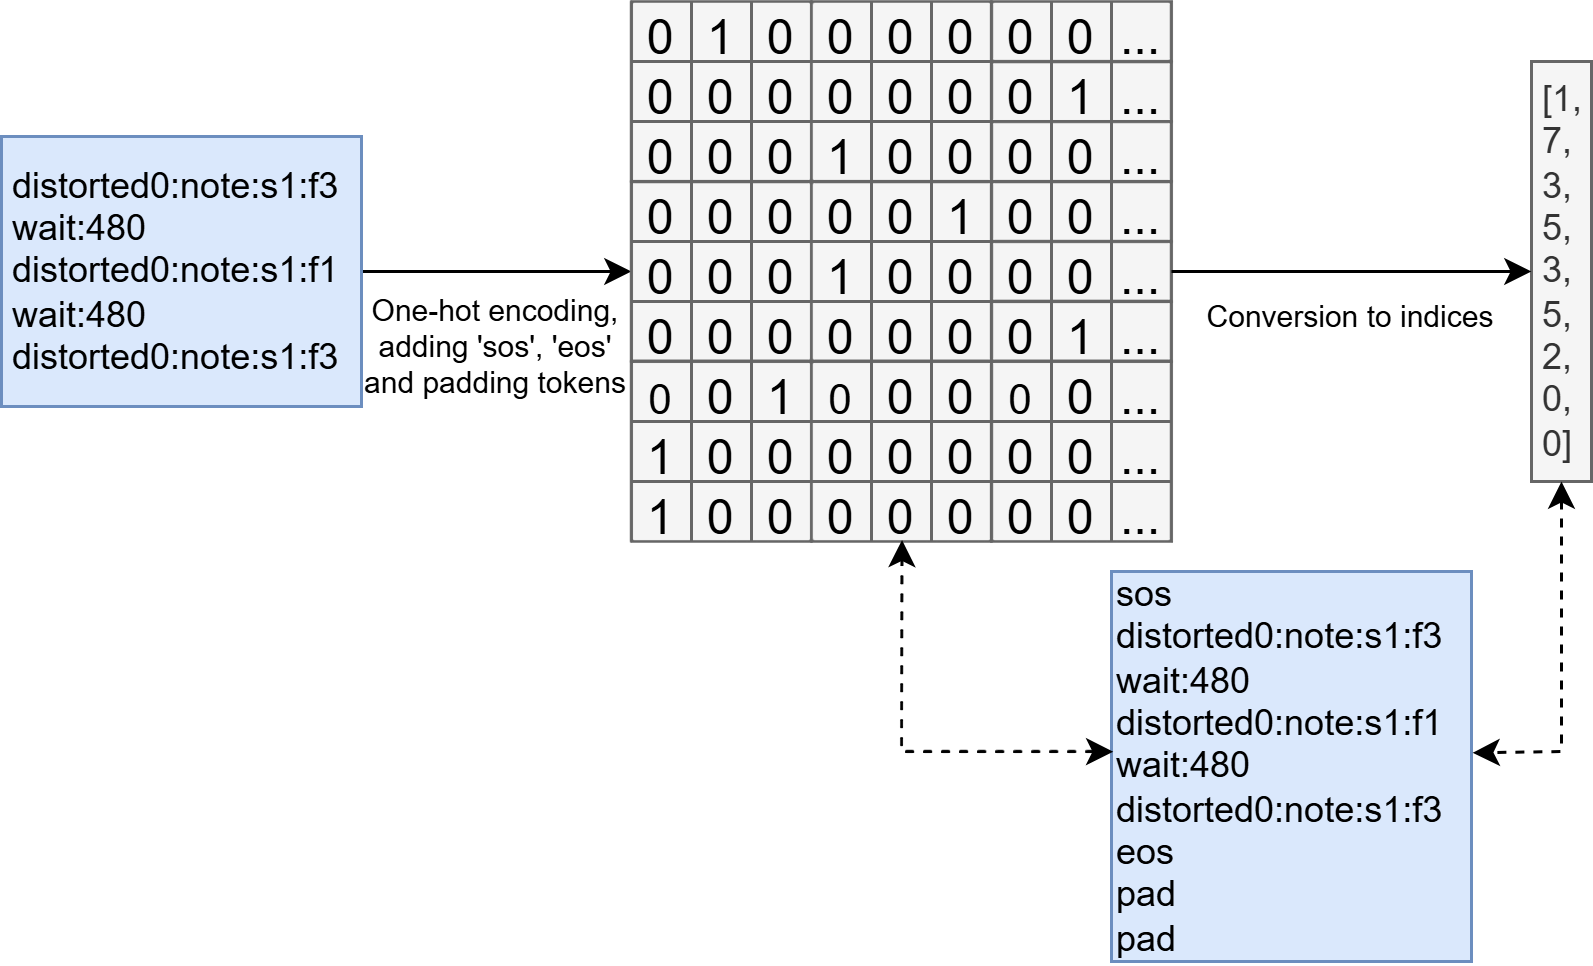
\includegraphics[width=.8\linewidth]{../images-figures/conversion_indices.png}
    \caption{Conversion from a txt token sequence to indices}
    \label{fig:conversion_indices}
\end{figure}

The sequences are then processed as described in Figure~\ref{fig:conversion_indices}.
They go through a one-hot encoding process, then we add 'start of sequence' and 'end of sequence',
and padding tokens after the 'eos' token to reach a fixed length of 797 tokens for the encoder (Rhythm guitar) and 773 tokens for the decoder (Bass guitar).
The final dictionary of sequences as indices is finally split into training, validation and test sets with proportions 0.8, 0.1 and 0.1 respectively.
We generated 118 167 sequences in total, which leads to 94 533 sequences in the training set and 11 817 in both the validation and test sets.
Those sets are respectively used to train the model, tune the hyperparameters and evaluate the model's performance.

